\chapter{Архитектура и реализация программного комплекса для моделирования поверхностных волн методом SPH}

Программный комплекс для решения задач вычислительной гидродинамики методом сглаженных частиц (SPH) 
обладает модульной архитектурой и состоит из следующих основных компонентов:
%
\begin{enumerate}
    \item вычислительный модуль (\verb|RRSPH|), включающий несколько реализаций с различными методами параллелизации:
        \begin{itemize}
            \item \verb|RRSPH_CL| (реализация на OpenCL);
            \item \verb|RRSPH_OMP| (реализация на OpenMP);
        \end{itemize}
    \item модуль визуализации:
        \begin{itemize}
            \item \verb|SPH2D_Drawer| (2D-визуализация);
            \item \verb|Scatter3D| (3D-визуализация);
        \end{itemize}
    \item аналитический модуль:
         \begin{itemize}
            \item \verb|FuncAtPoint| (анализ характеристик поля);
            \item \verb|WaterProfile| (построение профилей).
        \end{itemize}
\end{enumerate}

Перспективным направлением развития является интеграция всех компонентов в единую программную платформу \verb|RRSPH|.
%
При разработке использовались стандарты C++17 и C++20~\cite{Gregoire2021, Savitch2016}. 
%
Для обеспечения кроссплатформенности применена система сборки CMake~\cite{Swidzinski2022}.
%
Проведено тестирование сборки в следующих средах:
\begin{itemize}
    \item IDE: Microsoft Visual Studio Community 2019/2022, Visual Studio Code;
    \item компиляторы: MSVC, Clang, MinGW GCC;
    \item системы: Windows 10/11, Linux (Ubuntu, Manjaro, Fedora), WSL (Ubuntu).
\end{itemize}

%%%%%%%%%%%%%%%%%%%%%%%%%%%%%%%%%%%%%%%%%%%%%%%%%%%%%%%%%%%%%%%%%%%%%%%%%%%%%%%%%%%%%%%%%%%%%%%%%%%%%%
\section{Архитектура потоков данных в программном комплексе}
%%%%%%%%%%%%%%%%%%%%%%%%%%%%%%%%%%%%%%%%%%%%%%%%%%%%%%%%%%%%%%%%%%%%%%%%%%%%%%%%%%%%%%%%%%%%%%%%%%%%%%

На рисунке~\ref{f:dfd} представлена диаграмма потоков данных (DFD), 
иллюстрирующая архитектуру взаимодействия компонентов программного комплекса. 
%
Диаграмма включает:
\begin{itemize}
    \item основные потоки данных;
    \item процессы обработки;
    \item хранилища данных.
\end{itemize}
%
\begin{figure}[h!]
    \centering
    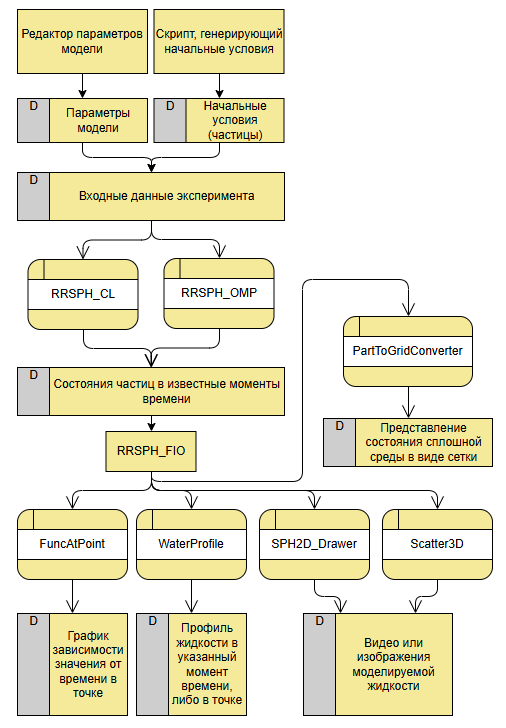
\includegraphics[width=0.8\textwidth]{images/dfd2025.png}
    \caption{Диаграмма потоков данных программного комплекса RRSPH.}
    \label{f:dfd}
\end{figure}
%
Процесс моделирования задаётся с помощью файла с исходными данными эксперимента (\verb|Params.json|).
Далее происходит моделирования жидкости выбранной программой. 

Результатом моделирования являются файлы, содержащие список всех частиц: их состояние и координаты. 
Каждый файл описывает отдельный временной слой, в названии указывается его номер.
Файлы структурированы как таблицы csv.

Данные временных слоёв хранятся в формате CSV и обрабатываются специализированной библиотекой \verb|RRSPH_FIO|.

Аналитические модули выполняют следующие функции:
\begin{itemize}
    \item \verb|FuncAtPoint| --- вычисление временных зависимостей характеристик поля в заданной точке;
    \item \verb|WaterProfile| --- построение пространственных или временных профилей жидкости.
\end{itemize}

Модуль \verb|SPH2D_Drawer| обеспечивает:
\begin{itemize}
    \item визуализацию частиц;
    \item генерацию тепловых карт;
    \item создание анимационных последовательностей (с помощью ffmpeg).
\end{itemize}

Для преобразования частичного представления в сеточное используется модуль \verb|PartToGridConverter|, 
результаты которого визуализируются посредством \verb|2DGrid_Drawer|.

Существуют также конфигурационные файлы, регулирующие работу приложений, которые не отображены на диаграмме. 
Каждое приложение может использовать такой файл для быстрого изменения своего поведения.

%%%%%%%%%%%%%%%%%%%%%%%%%%%%%%%%%%%%%%%%%%%%%%%%%%%%%%%%%%%%%%%%%%%%%%%%%%%%%%%%%%%%%%%%%%%%%%%%%%%%%%
\section{Вычислительная часть комплекса ПО для моделирования динамики жидкости}
%%%%%%%%%%%%%%%%%%%%%%%%%%%%%%%%%%%%%%%%%%%%%%%%%%%%%%%%%%%%%%%%%%%%%%%%%%%%%%%%%%%%%%%%%%%%%%%%%%%%%%

За основу приложения для вычислений был взят исходный код <<A 3D SPH code for solving the N-S equations>> 
из книги <<Smoothed Particle Hydrodynamics. A Meshfree Particle Method~\cite{Liu2003}>> 
на языке Fortran (использование свободное, если есть ссылка на источник).
Код был переведён на C++, после чего был адаптирован под поставленные задачи.

Разработанные программы используют параллельные технологии OpenMP и OpenCL, 
что позволяет значительно ускорить процесс вычислений, 
так как моделирование динамики жидкости методом SPH является задачей массового параллелизма.

%%%%%%%%%%%%%%%%%%%%%%%%%%%%%%%%%%%%%%%%%%%%%%%%
\subsection{Разбиение вычислительной части ПО на модули}
%%%%%%%%%%%%%%%%%%%%%%%%%%%%%%%%%%%%%%%%%%%%%%%%

В программе \verb|RRSPH_OMP| 11 модулей написанных в процедурном стиле:
%
\begin{enumerate}
    \item[1)] \verb|TimeIntegration| (шаги и полушаги по времени);
    \item[2)] \verb|UpdateAcceleration| (пересчёт всех параметров для одного шага по времени);
    \item[3)] \verb|SmoothingKernel| (ядра сглаживания);
    \item[4)] \verb|Density| (вычисление плотности с помощью уравнения непрерывности, либо сглаживанием массы);
    \item[5)] \verb|InternalForce| (внутренние силы --- вязкость и давление);
    \item[6)] \verb|ArtificialViscosity| (искусственная вязкость);
    \item[7)] \verb|ExternalForce| (внешние силы --- сила тяжести и силы взаимодействия с границами);
    \item[8)] \verb|AverageVelocity| (усреднение скорости);
    \item[9)] \verb|WaveMaker| (генераторы волн);
    \item[10)] \verb|EOS| (уравнения состояния);
    \item[12)] \verb|Searching| (NNPS, поиск пар взаимодействющих частиц напрямую, либо с помощью сетки).
\end{enumerate}

Блок-схема, описывающая процесс вычислений представлена на рисунке~\ref{f:SPH2D_scheme1}.
%
\begin{figure}[h!]
    \centering
    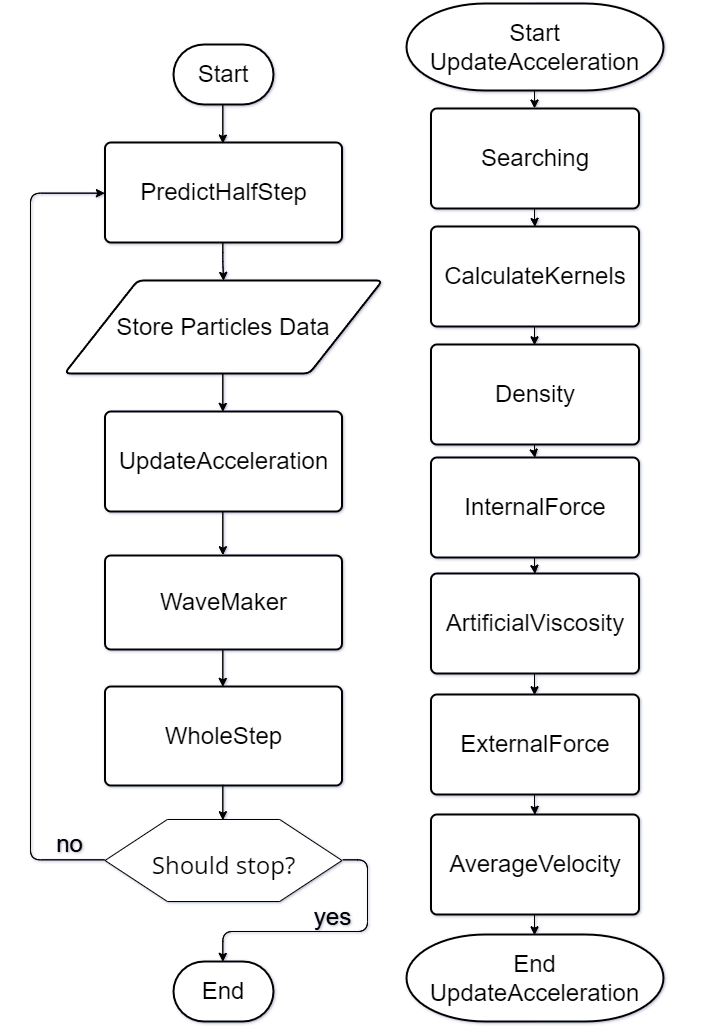
\includegraphics[width=0.65\textwidth]{images/SPH2D_scheme.png}
    \caption{Блок-схема, описывающая процесс вычислений}
    \label{f:SPH2D_scheme1}
\end{figure}
%
На ней изображены основные вызываемые в процессе вычислений функции, из которых большинство является отдельными модулями. 
Все программы для вычислений из разработанного комплекса ПО в целом сохраняют указанную структуру рассчётов и деление на модули, 
меняется реализация модулей.

%%%%%%%%%%%%%%%%%%%%%%%%%%%%%%%%%%%%%%%%%%%%%%%%
\subsection{Содержание общих модулей программ для вычислений}
%%%%%%%%%%%%%%%%%%%%%%%%%%%%%%%%%%%%%%%%%%%%%%%%

В модуле \verb|TimeIntegration| выполняется интегрирование по времени, 
левая часть блок-схемы на рисунке~\ref{f:SPH2D_scheme1} реализована в нём.

Интегрирование выполняется с помощью метода Leapfrog, по формуле~\ref{eq:leapfrog} с небольшими модификациями~\cite{Liu2003}.
Первый шаг делается отдельно, по системе~\ref{eq:leapfrog0}.
%
\begin{equation}\label{eq:leapfrog0}
    \begin{cases}
        t = t_{0} + \Delta t, 
        \\
        \rho_{i}(t_{0} + 0.5 \Delta t) = \rho_{i}(t_{0}) + 0.5 \Delta t \cdot D\rho_{i}(t_{0}),
        \\
        \vec{v}_{i}(t_{0} + 0.5 \Delta t) = \vec{v}_{i}(t_{0}) + 0.5 \Delta t  \cdot D\vec{v}_{i}(t_{0}),
        \\
        \vec{r}_{i}(t_{0} + \Delta t) = \vec{r}_{i}(t_{0}) + \Delta t \cdot \vec{v}_{i}(t_{0}+0.5\Delta t).
    \end{cases} 
\end{equation}
%
Далее входим в итерационный процесс.
Делаем полшага для плотности и скорости в функции \verb|PredictHalfStep| по формуле~\ref{eq:leapfrog1}.
%
\begin{equation}\label{eq:leapfrog1}
    \begin{cases}
        \rho_{i}(t) = \rho_{i}(t - 0.5 \Delta t) + 0.5 \Delta t \cdot D\rho_{i}(t - \Delta t),
        \\
        \vec{v}_{i}(t) = \vec{v}_{i}(t - 0.5 \Delta t) + 0.5 \Delta t \cdot D\vec{v}_{i}(t - \Delta t).
    \end{cases} 
\end{equation}
%
После этого вычисляем производные для момента времени $t$, и делаем полный шаг по системе~\ref{eq:leapfrog2} в функции \verb|WholeStep|.
%
\begin{equation}\label{eq:leapfrog2}
    \begin{cases}
        t = t + \Delta t, 
        \\
        \rho_{i}(t + 0.5 \Delta t) = \rho_{i}(t - 0.5 \Delta t) + \Delta t \cdot D\rho_{i}(t),
        \\
        \vec{v}_{i}(t + 0.5 \Delta t) = \vec{v}_{i}(t - 0.5 \Delta t) + \Delta t \cdot D\vec{v}_{i}(t),
        \\
        \vec{r}_{i}(t + \Delta t) = \vec{r}_{i}(t) + \Delta t \cdot \vec{v}_{i}(t+0.5\Delta t).
    \end{cases} 
\end{equation}

Итерационный процесс прекращается, когда $t \geq t_{\text{max}}$, и моделирование заданного интервала времени завершено.

Разные вычислительные модули могут использовать разные сглаживающие ядра. 
К примеру, \verb|Density| нужно гладкое ядро, такое как кубический сплайн (\ref{eq:w_cubic}), 
\verb|InternalForce| и \verb|ArtificialViscosity| лучше подходит негладкое ядро (\ref{eq:w_desbrun}), 
а \verb|AverageVelocity| требует отличное от используемых в уравнениях сохранения ядро.
За сглаживающие ядра отвечает модуль \verb|SmoothingKernel|.

Каждому ядру поставлен в соответствие идентификатор, 
с помощью которого производится поиск и рассчёт всех требуемых ядер и переиспользование результатов вычислений в случае, 
если некоторые модули используют одно и то же ядро.

На данный момент для выбора доступны ядра \ref{eq:w_gauss}, \ref{eq:w_cubic}, \ref{eq:wendland} и \ref{eq:w_desbrun}.

Общий код для вычислений выделен в отдельный файл, 
который используется всеми программами для вычислений и написан на C из-за ограничений языка OpenCL C.

В модуле \verb|Density| реализованы оба подхода к моделированию плотности: 
SPH-суммирование (\ref{eq:sum_density}) и интегрирование уравнения непрерывности (\ref{eq:continuity}).
%
Для решения проблемы с плотностью на границах можно подключать нормализацию по формуле \ref{eq:nor_density}.

Модуль \verb|InternalForce| предназначен для рассчёта части уравнения движения частиц, а именно:
%
\begin{equation}
    \frac{D\vec{v}_{i}}{Dt} = -\sum\limits_{j}m_{j}\left(
    \frac{p_{j}}{\rho_{j}^{2}} +
    \frac{p_{i}}{\rho_{i}^{2}}
    \right) \nabla_{i} W_{ij} + \vec{g} + F^{(visc)}.
\end{equation}
%
Это наиболее времязатратная часть вычислительных программ данного комплекса ПО.
Представлена возможность смены способа вычисления выражения в скобках на другое представление:
%
\begin{equation}
    \frac{D\vec{v}_{i}}{Dt} = -\sum\limits_{j}m_{j}\left(
    \frac{p_{j} + p_{i}}{\rho_{j}\rho_{i}}
    \right) \nabla_{i} W_{ij} + \vec{g} + F^{(visc)}.
\end{equation}
%
Также есть возможность включить или отключить вычисление вязкости, задания коэффициента динамической вязкости.
%
И здесь же реализован расчёт искусственного давления, если оно необходимо.

В модулях \verb|ArtificialViscosity| и \verb|AverageVelocity| производится рассчёт искусственной вязкости по формуле~\ref{eq:art_visc} 
и усреднение скорости формулей~\ref{eq:xsph} соответственно.

Оба численных модификатора можно отключить, а также поменять их свободные параметры 
(изменение параметров искусственной вязкости повлечёт за собой изменение шага по времени).

Модуль \verb|ExternalForce| отвечает за применение граничных условий. 
На данный момент реализован метод динамических частиц, а также гибрид динамических и отталкивающих частиц, 
где отталкивающая сила рассчитывается по формуле \ref{eq:sbt1}.
Реализована возможность выбора граничных условий, толщины стенок и расстояния между граничными частицами. 

Добавлена возможность включать генератор волн, реализованный в модуле \verb|WaveMaker|. 
В полной мере реализован метод динамических границ, заключающийся в моделировании движения поршня.
%
Чтобы созданные волны были более гладкими, генератор волн включается не сразу, а с задержкой, 
необходимой для того, чтобы частицы успели прийти в равновесие.
%
Более того, качество волн улучшает модель генератора волн второго порядка.

%%%%%%%%%%%%%%%%%%%%%%%%%%%%%%%%%%%%%%%%%%%%%%%%
\subsection{Модули поиска пар взаимодействующих частиц}
%%%%%%%%%%%%%%%%%%%%%%%%%%%%%%%%%%%%%%%%%%%%%%%%

В исходном коде на Fortran был реализован метод полного перебора всех частиц \verb|DirectFind|, 
но он обладает сложностью $O(N^2)$, и может применяться, когда число частиц порядка сотен или тысячи.

Чтобы ускорить поиск взаимодействующих частиц, предложены различные методы поиска. 

Чаще всего используют сеточные методы, 
которые очень просто можно распараллелить~\cite{Xia2016, Morillo2015, Nie2014, Monaghan1985}. 
Они хорошо подходят в том случае, когда длина сглаживания $h$ не зависит от координаты, например, при моделировании несжимаемых сред. 
И в случае, когда число частиц в ячейках мало, сложность сеточного алгоритма поиска оказывается порядка $O(N)$, 
что делает их наиболее быстрыми~\cite{Gross2019}.

Если длина сглаживания меняется в пространстве, что обычно применяется при моделировании газов, 
то лучше применять бинарные деревья (квадро- или октарные деревья на плоскости и в пространстве соответственно), 
либо другие виды деревьев~\cite{Xia2016}.
Он заключается в разбиении моделируемой области на отрезки (квадраты или кубы) до тех пор, 
пока листьями дерева не окажутся одиночными частицы.
Такие алгоритмы обычно обладают сложностью $O(N\log N)$ и требуют динамического выделения памяти при построении 
(либо их использование становится очень сложным), что особенно сложно при вычислениях на GPU~\cite{Gross2019}.

В \verb|RRSPH_OMP| реализован последовательный алгоритм создания сетки, 
так как переключение между одним или несколькими потоками происходит быстро, и алгоритм оказывается простым.

Массив номеров частиц \verb|grid|, отсортированный по номеру ячейки, в которой находится частица, 
а также индекс по этому массиву --- массив ячеек \verb|cells|, в котором находятся индексы в \verb|grid|, 
по которому начинаются частицы из данной ячейки.
Фактически массив \verb|cells| --- это промежуточная структура данных, хэш-таблица, 
создаваемая в процессе сортировки частиц методом подсчёта (counting sort), 
но она понадобится далее, для обхода соседних ячеек при поиске.

Координаты ячейки, в которой находится частица, тривиален, так как известны границы моделируемой области и размеры ячейки --- $kh$, 
где $h$ --- длина сглаживания, а $k$ --- коэффициент дальнодействия ядра 
(для Гауссова ядра это 3, для остальных ядер, описанных в данной работе, это 2). 
На рисунке~\ref{f:searchcells} представлена сетка для поиска взаимодействующих частиц, 
и область, в которой будет производиться поиск для чёрной частицы закрашена.
%
\begin{figure}[h!]
    \centering
    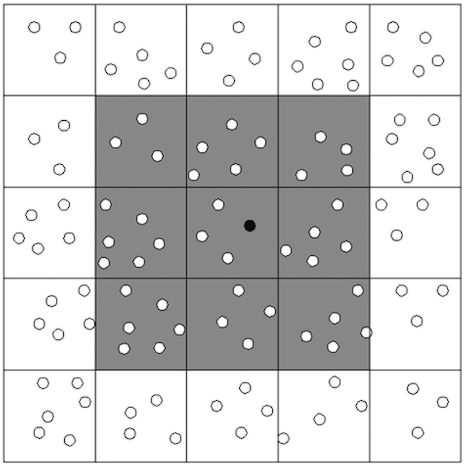
\includegraphics[width=0.5\textwidth]{images/cells_to_search.png}
    \caption{Сетка для поиска пар взаимодействующих частиц~\cite{Xia2016}}
    \label{f:searchcells}
\end{figure}
%
Чтобы можно было охарактеризовать ячейку одним числом (хэшем), 
вместо двух или трёх при многомерной задаче, используются кривые, заполняющие пространство по известному закону --- кривые Мортона, 
или $z$-кривые~\cite{Xia2016}.

Сортировка подсчётом плохо распараллеливается, 
а копирование координат частиц с памяти GPU в оперативную память и списки взаимодействующих частиц обратно --- дорогостоящая операция, 
поэтому реализована параллельная сортировка на GPU.

Из-за отсутствия промежуточной структуры данных, которая могла бы использоваться, 
как хэш-таблица, массив \verb|cells| вычисляется отдельно: 
с помощью бинарного поиска для каждой ячейки в данном массиве находим первую частицу, которая входит в неё.

Данный метод алгоритм используется в параллельной вычислительной программе, выполняющейся на GPU, \verb|RRSPH_CL|.

Далее кратко описан алгоритм поиска пар взаимодействующих частиц по сетке.
С помощью массивов \verb|grid| и \verb|cells| производится параллельный поиск соседних частиц для каждой частицы. 
Из координат данной частицы получаем координаты и номер ячейки, в которой она находится.
Из координат ячейки можно получить координаты и номера соседних ячеек, в которых будем искать соседние частицы.

Так как частицы из одной ячейки находятся последовательно в массиве \verb|grid|, 
с помощью индекса, хранящегося в \verb|cells|, можно обойти все частицы из данной ячейки, 
проверяя, что у очередной частицы номер ячейки не поменялся.
Так можно обойти все частицы из закрашенной области на рисунке~\ref{f:searchcells}.
Частицы взаимодействуют только в том случае, если находятся на расстоянии менее $kh$. 
После этой проверки можно добавлять очередную частицу в список соседей для данной частицы.

%%%%%%%%%%%%%%%%%%%%%%%%%%%%%%%%%%%%%%%%%%%%%%%%
\subsection{Модуль ввода-вывода для вычислительных программ комплекса}
%%%%%%%%%%%%%%%%%%%%%%%%%%%%%%%%%%%%%%%%%%%%%%%%

Данный модуль отвечает за взаимодействие с пользователем, а также за ввод-вывод данных о частицах.

Используется интерфейс командной строки, позволяющий в форме диалога задать название эксперимента, 
после чего будут созданы все необходимые директории и конфигурационные файлы, 
которые при дальнейшей разработке должны стать конфигурационными файлами проекта, и запускается рассчёт.
%
Если программе удаётся найти эксперимент с указанным именем, то предлагается его продолжить, 
начать с указанного временного слоя, либо заново с теми же начальными условиями.
%
В процессе рассчёта, который может занимать дни и недели, 
выводится затраченное время и предполагаемое время завершения в наиболее удобном масштабе.

Вывод данных о частицах производится в отдельных потоках, 
что позволяет не останавливать вычисления при записи на диск, что является очень медленной операцией.

Модуль чтения данных о частицах использует многопоточность (OpenMP) и проецирование файлов в память (библиотека \verb|mio|), 
что на быстрых дисках (SSD) позволяет увеличить скорость чтения в разы, 
что особенно важно, когда данных становится много, и они занимают гигабайты.

%%%%%%%%%%%%%%%%%%%%%%%%%%%%%%%%%%%%%%%%%%%%%%%%%%%%%%%%%%%%%%%%%%%%%%%%%%%%%%%%%%%%%%%%%%%%%%%%%%%%%%
\section{Визуальная часть комплекса ПО для моделирования поверхностных волн}
%%%%%%%%%%%%%%%%%%%%%%%%%%%%%%%%%%%%%%%%%%%%%%%%%%%%%%%%%%%%%%%%%%%%%%%%%%%%%%%%%%%%%%%%%%%%%%%%%%%%%%

Часто требуется визуализировать результаты анализа данных, полученных во время моделирования. 
%
Они обычно представляют собой таблицы координат и значений функции по данным координатам.
%
Для их визуализации используется пакет \verb|GnuPlot|, позволяющий строить графики по точкам.
% 
Он нужен для гибкой настройки одномерных графиков, полученных в результате обработки полученных данных. 
%
Помимо файлов с данными аналитические программы генерируют скрипты для \verb|GnuPlot|, 
чтобы можно было быстро настроить и построить графики.

Чтобы визуализировать данные в более сложной форме требуется соответствующе программное обеспечение, которое описано ниже.

\subsection{Средство визуализации частиц SPH2D\_Drawer}

Программа для моделирования выдаёт данные в виде множества файлов, 
в которых описано состояние всех частиц для всех слоёв, кратных шагу сохранения.
%
В самом простом случае требуется вывести положение частиц среды в разные моменты времени. 
%
Может потребоваться вывести свойства частиц в виде их цвета, тогда строится тепловая карта.
%
Для вывода таких данных в виде частиц используется \verb|SPH2D_Drawer|.

Эта программа была разработана на языке C++ 20 стандарта~\cite{Gregoire2021} 
с использованием графической библиотеки \verb|SDL2|~\cite{Mitchell2013}, 
библиотеки \verb|nlohman/json| для чтения файла конфигурации и 
библиотеки \verb|csv-parser| для быстрого чтения данных с помощью проецирования файла в память.
%
За основу были взяты наработки в области разработки игр на \verb|SDL2|~\cite{Mitchell2013}. 
Программа разделена на составляющие, отвечающие за данные, выводимые на экран, 
обработку ввода в реальном времени и сам вывод на экран --- по схеме Model-View-Controller.

Существует возможность масштабирования, перемещения по координатам, перемещения по времени, проигрывания анимации динамики жидкости, 
регулировка скорости проигрывания, приостановки, записи видео или отдельных кадров с помощью горячих клавиш.

Для более тонкой настройки добавлена система команд, позволяющая редактировать большинство переменных.
%
Чтобы ускорить настройку отображения результатов моделирования, добавлена возможность загружать настройки из файлов конфигурации.

Помимо самих частиц выводится время от начала эксперимента, а также легенда, если включена тепловая карта.
%
Тепловая карта позволяет выбрать, по какому свойству задавать цвет частицы, а также границы этого свойства.

\subsection{Визуализация среды с помощью сетки в программе 2DGrid\_Drawer}

Использование программы для визуализации частиц \verb|SPH2D_Drawer| показало, что у неё есть очевидные границы применимости. 
При небольшом количестве частиц --- до сотни тысяч, и объёме данных до нескольких гигабайт, она отлично справляется со своей задачей.
Но при визуализации миллиона частиц возникли проблемы с производительностью.
Результаты моделирования четырёх миллионов частиц не поместились в 16Гб оперативной памяти, 
а один кадр отрисовывался порядка десяти секунд.
Эти проблемы не позволяют использовать данную программу как средство визуализации в режиме реального времени для мастабных экспериментов.

Данную задачу позволяет решить использование сетки.
В таком случае не будет зависимости объёмов данных и времени процессора от количества частиц. 
Вместо этого будет зависимость только от количества узлов в сетке, которое может быть одинаковым, 
как при тысяче частиц, так и при миллионах.

Перед визуализацией нужно получить представление жидкости в виде сетки. 
Для этого используется программа \verb|PartToGridConverter|. 
Она принимает на вход частицы и исходные параметры и преобразует их в сетку с заданным шагом дискретизации.
Для преобразования используется формула~\ref{eq:sph_approx}, где индекс $i$ обозначает узлы сетки.
На выходе программа генерирует файлы, представляющие жидкость в виде сетки с некоторыми свойствами в узлах.

Далее результаты моделирования в данном представлении могут быть визуализированы с помощью программы \verb|2DGrid_Drawer|.
Если на вход этой программе даны результаты моделирования в виде частиц, то она автоматически вызовет их конвертацию в сетку. 

%%%%%%%%%%%%%%%%%%%%%%%%%%%%%%%%%%%%%%%%%%%%%%%%%%%%%%%%%%%%%%%%%%%%%%%%%%%%%%%%%%%%%%%%%%%%%%%%%%%%%%
\section{Аналитическая часть комплекса ПО для моделирования поверхностных волн}
%%%%%%%%%%%%%%%%%%%%%%%%%%%%%%%%%%%%%%%%%%%%%%%%%%%%%%%%%%%%%%%%%%%%%%%%%%%%%%%%%%%%%%%%%%%%%%%%%%%%%%

%%%%%%%%%%%%%%%%%%%%%%%%%%%%%%%%%%%%%%%%%%%%%%%%
\subsection{Программа для определения значения функции в точке}
%%%%%%%%%%%%%%%%%%%%%%%%%%%%%%%%%%%%%%%%%%%%%%%%

Программа \verb|FuncAtPoint| разработана для определения значения функции в указанной точке с течением времени.
%
Ей на вход подаются результаты моделирования в виде частиц, и с помощью формулы~\ref{eq:sph_approx} 
на каждом временном слое определяется значение указанной функции.

В программе используется интерфейс в виде консоли (CLI), 
либо можно передать необходимые параметры с помощью аргументов при вызове.
Для обработки переданных аргументов используется библиотека \verb|cxxopts|, 
позволяющая использовать, как именованные, так и неименованные аргументы.

\subsection{Программа для опеределения профиля жидкости}

При моделировании волн на поверхности воды часто требуется определить её глубину в каждой точке пространства.
Либо дана точка, и нужно определить зависимость глубины воды в этой точке от времени.

Эти задачи позволяет решить программа \verb|WaterProfile|. 
%
Ей на вход подаются результаты моделирования в виде частиц, после чего для каждого исследуемого момента времени, 
в некотором радиусе от заданной точки производится поиск нескольких частиц с наибольшей высотой.
%
С помощью сглаживания по ним определяется глубина в данной точке.
%
Данная задача является задачей массового параллелизма, а потому в программе повсеместно используется OpenMP.

В отличие от \verb|FuncAtPoint|, здесь не используется CLI, а все параметры для анализа передаются с помощью конфигурационного файла, 
что в дальнейшем позволит использовать данную программу как сервис для других частей программного комплекса.

\FloatBarrier
